%%%%%%%%%%%%%%%%%%%%%%%%%%%%%%%%%%%%%%%%%%%%%%%%%%%%%%%%%%%%%%%%%%%%%%%%%%%%%%
%%
%% Dokumentacia k projektu 'Interpret pre jazyk IFJ 2013'
%%
%%
%%%%%%%%%%%%%%%%%%%%%%%%%%%%%%%%%%%%%%%%%%%%%%%%%%%%%%%%%%%%%%%%%%%%%%%%%%%%%%
\documentclass[12pt,a4paper,titlepage,final]{article}

% jazyk
\usepackage[slovak]{babel}
\usepackage[utf8]{inputenc}
% balicky prr odkazy
\usepackage[bookmarksopen,colorlinks,plainpages=false,urlcolor=blue,unicode]{hyperref}
\usepackage{url}
% obrazky
\usepackage[dvipdf]{graphicx}
% velikost stranky
\usepackage[top=3.5cm, left=2.5cm, text={17cm, 24cm}, ignorefoot]{geometry}

\setcounter{secnumdepth}{4}
\usepackage{pdflscape}
\usepackage{afterpage}
\usepackage{capt-of}% or use the larger `caption` package

\begin{document}

%%%%%%%%%%%%%%%%%%%%%%%%%%%%%%%%%%%%%%%%%%%%%%%%%%%%%%%%%%%%%%%%%%%%%%%%%%%%%%
% titulní strana

\def\projname{Dokumentácia IFJ 2013}


\begin{titlepage}

% \vspace*{1cm}
\begin{figure}[!h]
  \centering
  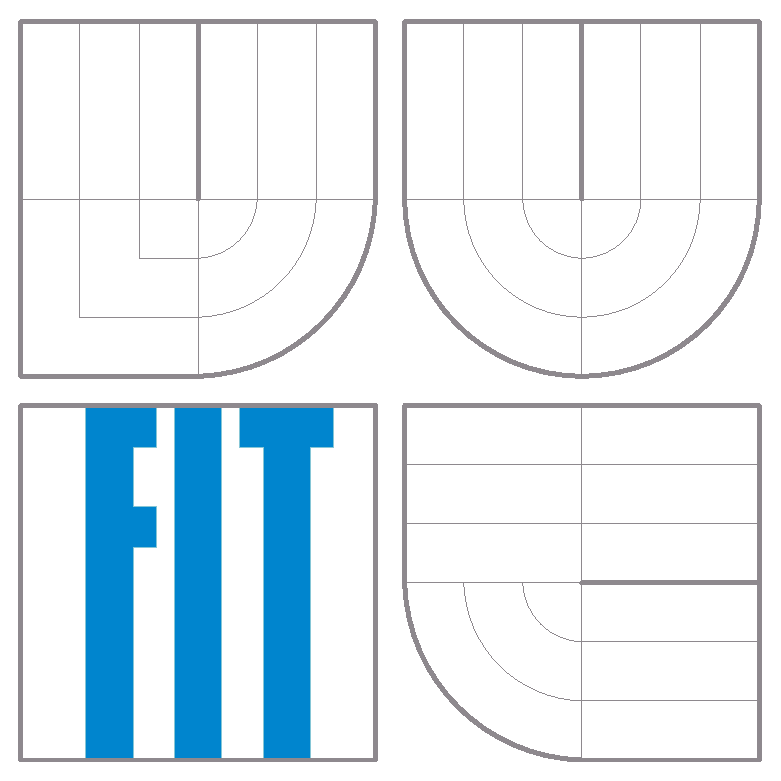
\includegraphics[height=5cm]{doc/img/logo.eps}
\end{figure}
\center Fakulta Informačních Technologií \\
\center Vysoké Učení Technické v Brně \\

\vfill

\begin{center}
\bigskip
\begin{Huge}
\projname\\
\end{Huge}
\begin{large}
Varianta a/4/II
\end{large}
\end{center}

\vfill

\begin{center}
\begin{Large}
\today
\end{Large}
\end{center}

\vfill

\begin{flushleft}
\begin{large}
Team leader: Marek Milkovič (xmilko01), 20\% \\
Členovia: Lukáš Vrabec (xvrabe07), 20\% \\
\hspace{57px} Ján Spišiak (xspisi03), 20\% \\
\hspace{57px} Ivan Ševčík (xsevci50), 20\% \\
\hspace{57px} Marek Bertovič (xberto00), 20\% \\ 
\end{large}
\end{flushleft}
\end{titlepage}

%%%%%%%%%%%%%%%%%%%%%%%%%%%%%%%%%%%%%%%%%%%%%%%%%%%%%%%%%%%%%%%%%%%%%%%%%%%%%%
% obsah
\pagestyle{plain}
\pagenumbering{roman}
\setcounter{page}{1}
\tableofcontents

%%%%%%%%%%%%%%%%%%%%%%%%%%%%%%%%%%%%%%%%%%%%%%%%%%%%%%%%%%%%%%%%%%%%%%%%%%%%%%
% textova zprava
\newpage
\pagestyle{plain}
\pagenumbering{arabic}
\setcounter{page}{1}

%%%%%%%%%%%%%%%%%%%%%%%%%%%%%%%%%%%%%%%%%%%%%%%%%%%%%%%%%%%%%%%%%%%%%%%%%%%%%%

% lex
%%%%%%%%%%%%%%%%%%%%%%%%%%%%%%%%%%%%%%%%%%%%%%%%%%%%%%%%%%%%%%%%%%%%%%%%%%%%%%
\section{Riešenie interpretu} \label{Riesenie interpretu}
%%%%%%%%%%%%%%%%%%%%%%%%%%%%%%%%%%%%%%%%%%%%%%%%%%%%%%%%%%%%%%%%%%%%%%%%%%%%%%

%=============================================================================
\subsection{Lexikálna analýza}
Úlohy lexikálnej analýzy sú:
\begin{enumerate}
    \itemsep0em
    \item čítanie znakov zo vstupu a ich preklad na postupnosť tokenov, ktoré ďalej slúžia syntaktickej analýze
    \item odstránenie komentárov a bielych znakov v zdrojovom programe
    \item nájdenie lexikálnych chýb v zdrojovom programe
\end{enumerate}

Výstup lexikálnej analýzy je zároveň vstupom do syntaktickej analýzy, preto je
lexikálna analýza volaná syntaktickou analýzou. V našom prípade je konkrétne
výstup lexikálnej analýzy vektor tokenov, kde token je štruktúra obsahujúca
informácie o type tokenu (typ tokenu je enumerácia všetkých prípustných tokenov)
a v prípade tokenov vyžadujúcich dalšie informácie ako napríklad obsah stringu
(znakový reťazec) čí číselnu hodnotu tokenu typu číslo obsahuje štruktúra aj tieto dáta.
Úlohou je teda prejsť celým súborom až pokým scanner nenájde koniec vstupného súboru
(v C terminológii \texttt{EOF} - End Of File), odhaliť prípadne lexikálne chyby a
v prípade lexikálnej bezchybnosti programu vyplniť vektor tokenmi a pripraviť
tak vstup do syntaktickej analýzy.

Implementácia lexikálnej analýzy spočíva v konštrukcii konečného automatu
(v angličtine finite state machine), ktorý prečíta znak zo súboru, vyhodnotí
ho a na základe aktuálneho stavu a vstupného znaku môžu nastať tri nasledujúce
 možnosti:

1. aktuálny stav neumožnuje pokračovať s daným vstupným znakom a ukončuje tak
jeden token, znak sa "vracia" naspäť do vstupného súboru, avšak v našom prípade
len uloženie do pomocnej premennej a uchovanie informácie, že další znak pre
další token bude čítaný nie zo súboru ale z tejto pomocnej premennej.

2. aktálny stav umožnuje pokračovať s daným vstupným znakom, mení sa stav automatu,
avšak táto zmena môže byť v niektorých prípadoch nie úplne zmenou ak pokračujeme
do stavu, ktorý je zároveň aktuálnym stavom.

3. aktuálny stav neumožnuje pokračovat s daným vstupným znakom a zároveň
nedovoluje ukončiť token.To znamená,že sa v programe nachádza lexikálna chyba.

Špeciálnym prípadom sú stavy pre komentáre a blokové komentáre programu, ktoré
lexikálna analýza registruje, ale kedže sú nepodstatné pre činnosť zdrojového
programu, zahadzuje tieto informácie a ani ich ďalej nespracúva a neposiela
syntaktickej analýze v podobe tokenu.

Tento automat najlepšie ilustruje príloha č.1, kde je nakreslený model
automatu lexikálnej analýzy.

%=============================================================================
\subsection{Syntaktická a sémantická analýza}
Syntaktická analýya sa spúšťa po lexikálnej analýze a pracuje s vektorom tokenov,
ktorý naplnila. Riadi LL gramatikou a jej pravidlami podľa LL tabuľky v prílohách.
Implementovaná je rekurzívnym zostupom, pričom v prípade vyhodnocovania výrazov sa
z nej spúšťa precedenčná analýza.

Vzhľadom na to, že nami implementovaný jazyk podporuje volanie funkcie ešte pred
jej definíciou, alebo napríklad deklaráciu premennej v podmienenej časti kódu,
použili sme dvojfázový priechod vektorom tokenov, kde pri prvom priechode sa zaznamenáva počet
lokálnych premenných v hlavnom tele programu a vo všetkých funkiách pričom tieto premenné
sú automaticky vkladané do lokálnych tabuliek symbolov a zároveň sa napĺňa aj globálna
tabuľka symbolov s definíciami funkcií. Pri druhom priechode preto už vieme, že či je daná funkcia
definovaná, alebo nie a na základe toho vrátiť správny chybový kód.

%=============================================================================
\subsection{Interpret}

%=============================================================================
\subsubsection{Vstupy}
Interpret je volaný s tromi parametrami:
\begin{enumerate}
    \itemsep0em
    \item Ukazateľ na prvú inštrukciu hlavného tela programu.
    \item Odkaz na tabuľku konštánt, kde sú uložené všetky konštantné hodnoty.
    \item Odkaz na tabuľku adries, ktorá poskytuje adresy na prvé inštrukcie funckií.
\end{enumerate}
Všetky parametre majú modifikátor \texttt{const}, chrániaci pred ich prípadnou zmenou
v rámci interpretácie. Inštrukcie sú v pameti uložené bezprostredne za sebou, čo
umožňuje jednoducho inkrementovať prvý predaný parameter po vykonaní aktuálnej
inštrukcie. Aj keď sú inštrukcie funkcií uložené oddelene od tých ktoré tvoria hlavné
telo programu, je možné sa k nim dostať práve cez reálne adresy uložené v tabuľke adries.

%=============================================================================
\subsubsection{Vnútorné štruktúry}

\paragraph{Zasobník}\mbox{}\\

Zásobník je najdôležitejšia štruktúra počas interpretácie. Je odvodená od štruktúry
\texttt{Vector}, no pre zrýchlenie interpretácie boli pre ňu implementované ďalšie
špecifické operácie. Rovnako ako tabuľka konštánt obsahuje položky typu \texttt{Value}, 
ktorý združuje typ a samotnú hodnotu. Na zásobníku sa môžu nachádzať premenné, parametre
funckie, referencie, zásobníkové a inštrukčné ukazatele ako aj medzivýsledky výrazov.

Kapacita zásobníku, tj. predalokované miesto, je v rámci optimalizácie nastavená pred
interpretáciou na dostatočne veľkú konštantu. Aj keď teda zásobník je dynamická štruktúra
s možnosťou zmeny svojej kapacity, reálne sa tak deje veľmi ojedinele, napríklad v programoch
využívajucich rekurziu.

\paragraph{Vektor}\mbox{}\\

\texttt{Vector} je najpoužívanejšou štruktúrou v rámci programu. Jedná sa o jednorozmerné pole s
dynamickou veľkosťou, uložené v pamäti ako jeden blok. Jeho prvky teda nasledujú v pamäti bezprostredne
za sebou. \texttt{Vector} obsahuje predalokovaný priestor o určitej veľkosti, nazývanej kapacita.
Ak by počet reálne využitých položiek, nazývaný veľkosť, mal presiahnuť kapacitu, vytvorí
sa nový blok v pamäti a dáta sa skopírujú z predchádzajúceho bloku, ktorý je následne uvoľnený.
Implementáciu tvoria dve časti -- všeobecná a špecifická.

Všeobecná časť definuje operácie, ktoré sú nezávislé od dátového typu položiek. Jedná sa napríklad
o operáciu \texttt{shrinkToFit}, ktorá obsah vektoru prealokuje do nového bloku, tak aby jeho
kapacita bola rovná veľkosti, čím sa uvoľní nevyužívaná pameť. 

Zdrojový kód pre špecifickú časť využíva makrá a definície, ktoré sa pred prekladom prepíšu
špecifickými názvami a kódom. Takto je možné zdielať jeden zdrojový kód pre všetky štruktúry,
ktoré majú vlastnosti štruktúry \texttt{Vector}, a líšia sa iba dátovým typom položiek. V hlavičkovom
súbore pre novú štruktúru sa zadefinuje s akým typom by mal \texttt{Vector} pracovať, 
a následne sú pre túto štruktúru nagenerované všetky potrebné operácie. Implementácia je možná vďaka
konvenciám pri vytváraní nových zložených typov a operácií nad nimi. V jazyku C++ sa pre tento účel
využívajú šablóny.

\texttt{Vector} je používaný ako základ väčšiny dynamických štruktúr, medzi ktoré patria napríklad:
\begin{itemize}
    \itemsep0em
    \item Zoznam tokenov
    \item Inštrukčný vektor
    \item Tabuľka symbolov
    \item Tabuľka konštánt
    \item Tabuľka adries
    \item Zásobník
\end{itemize}

%=============================================================================
\subsubsection{Inštrukcie}
Inštrukcia je reprezentovaná štruktúrou \texttt{Instruction}, ktorá obsahuje nasledujúce data:
\begin{itemize}
    \itemsep0em
    \item Inštrukčný kód
    \item Inštrukčný mód
    \item Operand A
    \item Operand B
    \item Operand R
\end{itemize}
Inštrukčný kód je reprezentovaný enumeráciou, podľa ktorej intepret vie, akú činnosť má vykonať pri
prečítaní danej inštrukcie. Inštrukčný mód je použitý pri niektorých inštrukciách, ktorých operand
môže byť buď konštanta z tabuľky konštánt alebo hodnota zo zásobnika, kde mód ako bitová maska
určuje, ktorý operand pochádza odkiaľ. Operandy A a B sú brané ako vstupné operandy do inštrukcie a sú
to čísla, ktoré informujú o pozícií v tabuľke konštánt. Operand R je braný ako cieľový a vyjadruje vždy
pozíciu na zásobníku v rámci aktuálneho zásobníkového ramca. Inštrukčná sada sa nachádza v prílohách.

%=============================================================================
\subsubsection{Činnosť}
Interpret má \texttt{instruction pointer} ukazujúci na inštrukciu v inštrukčnom vektore,
ktorá sa bude ako nasledujúca vykonávať. Po spustení interpretačnej časti programu
tento pointer ukazuje na prvú inštrukciu v hlavnom inštrukčnom vektore. Pokiaľ nedochádza ku skokom,
\texttt{instruction pointer} sa po inštrukčnom vektore posúva sekvenčne až na jeho koniec.

Pri skoku môže dôjsť k posunutiu \texttt{instruction pointer}a hocikde do hlavného
inštrukčného vektora, alebo aj do inštrukčného vektora pre funkcie v prípade volania funkcie.

Po inicializácií potrebných štruktúr a premenných sa začína interpretačný cyklus.
Ten prečíta z inštrukcie na ktorú ukazuje \texttt{instruction pointer} jej kód a podľa
toho reaguje svojou činnosťou. Na konci inštrukčného cyklu sa inkrementuje \texttt{instruction pointer},
ak zrovna nedošlo ku skoku.

Keď interpret rozpozná koniec programu na základe vložených inštrukcií a informáciam na zásobníku, svoju činnosť končí.

%=============================================================================
\subsubsection{Princípy}

\paragraph{Volanie funkcií}\mbox{}\\

Pred volaním funkcie musí byť na zásobniku zarezervované 1 miesto pre návratovú hodnotu.
Následné musia byť na zásobník vložené parametre funkcií v poradí, že prvý parameter bude
bezprostredne pred vykonaním inštrukcie pre zavolanie funkcie na vrchole zásobniku.

Po zavolaní funkcie sa na zásobníku interpretu vytvára zásobnikový ramec. Ten obsahuje (v tomto
poradí smerom k vyšším adresám) miesto pre návratovú hodnotu, parametre funkcie, starý \texttt{stack pointer}
, adresu inštrukcie pre návrat funkcie, lokálne premenné a zvyšok je určený pre medzivýsledky výrazov
a pre vytváranie ďaľších zásobnikových rámcov.

Ukončenie funkcie je sprevádzané nastavením \texttt{instruction pointer}a na adresu kam sa vykonávanie
programu vráti po zmazaní aktuálneho zásobníkového rámca. Následne je obnovený aj starý \texttt{stack
pointer} aby interpret ukazoval do nadradeného zásobníkového rámca a aktuálny zásobnikový
rámec je zničený.

\paragraph{Referencie}\mbox{}\\

V rámci optimalizácií interpret nepracuje vždy na zásobníku s konkrétnymi hodnotami,
ale aj s referenciami, čo sú ukazovatele na hodnoty niekde inde na zásobniku, poprípade
v tabuľke konštánt. Referencia má v sebe nesie informáciu o relatívnej vzdialenosti od miesta
na zásobníku, poprípade umiestnenie v tabuľke konštánt kam ukazuje. Existujú tieto typy referencií:

\begin{enumerate}
    \itemsep0em
    \item \texttt{Strong Reference}
    \item \texttt{Weak Reference}
    \item \texttt{Const Reference}
\end{enumerate}

Každá z nich má iné vlastnosti týkajúce sa toho kedy dochádza k dereferncií a kedy
je referencia prepísaná novou hodnotou.

\texttt{Strong Reference} sa používa pre návrátové hodnoty v prípade najvyššieho volanie funckie,
kedy sa do miesta pre návrtovú hodnotu vloží referencia na premennú do ktorej chceme
výsledok funkcie priradiť. Pri priradení do \texttt{Strong Reference} dochádza k dereferncií a teda
priamemu priradeniu bez zbytočných kopíí.

\texttt{Weak Reference} sa používa pre parametre funkcií, ktoré sú typu String, kvôli časovej náročnosti
kopírovania reťazca. Pri priradení do \texttt{Weak Reference} dochádza k nahradenie referencie
novou hodnotou predstavujúcou výsledok výrazu, ktorý bol priradený. Pri všetkých ostatných použitiach
\texttt{Weak Reference} dochádza k jej dereferencií. Pri snahe vložiť na zásobník referenciu na \texttt{Weak Reference}
je vytvorená \texttt{Weak Reference} na miesto kam ukazuje pôvodná \texttt{Weak Reference}.

\texttt{Const Reference} je referencia do tabuľky konštánt, chová sa presne tak isto ako \texttt{Weak Reference},
až na to že sa používa všade kde sa vo výraze nachádza konštanta.

%=============================================================================
\subsubsection{Vstavané funkcie}
Každá vstavaná funkcia predstavuje pre interpret samostatnú inštrukciu. Ak sa
názov vstavanej funkcie objaví vo výraze, je už za prekladu rozpoznaná a 
nageneruje sa príslušná inštrukcia. Vstavané funkcie zdieľajú koncept zásobníkového
rámca s užívateľom definovanými funkciami, teda na zásobníku sa pri zavolaní funkcie 
nachádza miesto pre návratovú hodnotu a následujú parametre. Keďže však vstavaná funkcia
má presne predpísanú činnosť, ktorá bola implementovaná ako súčasť interpretu v jazyku C,
nie je potrebné na zásobník ukladať \texttt{stack pointer} a \texttt{instruction pointer}.
Volanie vstavanej funkcie sa potom líši v tom, že namiesto \texttt{IST\_Call} sa vykoná 
príslušná inštrukcia vstavanej funckie a táto nastaví aj návratovú hodnotu.

Pre konverziu parametrov vstavaných funkcií na požadovaný typ sa využívajú už existujúce
konverzné funkcie, napríklad v prípade prevodu na \texttt{string} sa využije funkcia
\texttt{valueToString}, ktorá je však využitá aj pri vstavanej funkcii \texttt{strval}.
%%%%%%%%%%%%%%%%%%%%%%%%%%%%%%%%%%%%%%%%%%%%%%%%%%%%%%%%%%%%%%%%%%%%%%%%%%%%%%%

% IAL
%%%%%%%%%%%%%%%%%%%%%%%%%%%%%%%%%%%%%%%%%%%%%%%%%%%%%%%%%%%%%%%%%%%%%%%%%%%%%%
\section{Algoritmy} \label{Algoritmy}
%%%%%%%%%%%%%%%%%%%%%%%%%%%%%%%%%%%%%%%%%%%%%%%%%%%%%%%%%%%%%%%%%%%%%%%%%%%%%%

%=============================================================================
\subsection{Merge sort}
Na implementáciu radiaceho algoritmu sme využili Merge sort. Ide o radenie
 typu rozdeľuj a panuj (angl. divide and conquer), v našej implementácií stabilný
 algoritmus s časovou zložitosťou O(N log(N)). Princíp alogritmu je jednoduchý.
 Pole sa rozdelí na menšie podpolia (v našom prípade veľkosti 1). Následne sa
 po pároch spoja, tak aby výsledné pole bolo tiež zoradené.

Naša implementácia je tzv. zhora-dolu (angl. top-down) s pomocným poľom o
 rovnakej veľkosti ako zdrojové pole. Tieto polia striedajú svoju funkciu, z
 jedného sa číta do druhého píše, čím sa odstráni potreba kopírovania
 medzivýsledku spať do zdrojového poľa. Toto sa ľahko uskutoční jednoduchou
 zámenou argumentou v rekurzívnom volaní funkcie. Celá logika našej funkcie
 stringCharSortDivide() spočíva teda v rozdelení zdrojového poľa rekurzívnym
 volaním (s vymenením zdrojovým a cieľovým poľom) na polovice v prípade že jeho
 veľkosť je vačšia než 2, a následným spojením týchto 2 polovíc, pri ktorom sa
 vždy vyberie prvok podľa váhy z danej polovice.

% mozno obrazok sem dat? odpoved: NIE uz bez obrazkov to bude dost velke :D 

%=============================================================================
\subsection{KMP substring search}
Knuth-Morris-Prattov algoritmus zrýchľuje vyhľadávanie podreťazca v reťazci, za
 využita informácie o výskyte podreťazcov v hľadanom reťazci ktoré sa
 zhodujú so prefixom hľadaného reťazca. Túto informáciu bude držat pomocná
 tabuľka, ktorú musíme pred hľadaním zostaviť.

Základný vyhľadávací algoritmus porovnáva podreťazec s reťazcom postupne po
 každom znaku. KMP sa vyhýba porovaniu toho istého znaku v prípade že bol
 porovnaný predošlými porovnaniami a nie je možné aby bol súčasťou podreťazca
 ktorý je prefixom hľadaného reťazca. Samotné vyhľadávanie má teda zložitosť
 len O(N).

Naša pomocná tabuľka bude držať indexy, od ktorých musíme znova začať porovnávať.
 Zostavíme ju jednoducho postupným porovnávaním podreťazcou hľadaného reťazca s
 jeho prefixom. V prípade že neexistuje podreťazec o veľkosti väčšej než 1
 shodujúci sa so prefixom, bude tabuľka plná núl.

Vyhľadávanie je jednoduché, v prípade neshody sa podľa tabuľky nastaví ktorým
 písmenom z podreťazca sa má pokračovať porovnávanie.

%=============================================================================
\subsection{Hash table}
Hash tabuľka je typ abstraktnej dátovej štruktúry, ktorý implementuje operácie
 nad prvkami identifikovanými unikátnymi kľúčmi. Vyznačuje sa najmä časovou
 zložitosťou O(1).

V našej implementácií používame hash funkciu djb2 (autor Bernstein). Ide o
 pomerne jednoduchú a rýchlu funkciu, pričom vypočítaný hash ukladáme spolu so
 záznamom v tabuľke pre zrychlénie rekalkulácie pozície záznamu v prípade
 zmeny veľkosti tabuľky. Pri vyhľadavaní v tabuľke sa vypočíta hash z klúča,
 urobí sa modulo podľa veľkosti tabuľky (zvyčajne mocnina 2 takže vcelku rýchla
 operácia), pristúpi sa na daný prvok poľa kde sa zistí index záznamu (a v
 prípade že nastala kolízia, iteruje sa cez odkaz na ďalší záznam), pričom vždy
 sa musia porovnať porovnať klúče.

Interne naša tabuľka používa vektor na ukladanie záznamov. Takáto implementácia
 šetrí pamäť a zrýchľuje zmenu veľkosti tabuľky no nevýhodou je väčšia záťaž na
 cache procesoru (taktiež operácia mazania záznamu by bola komplikovanejšia,
 pokiaľ by sme ju implementovali). Pri kolízií uložíme do predošlého záznamu
 odkaz na ďaľší záznam.

Zmena veľkosti tabuľky sa deje pri záťaži 0,75. Zahodí sa staré pole indexov a
 alokuje sa dvojnásobne väčšie. Následne sa postupne vkladajú všetky odkazy na
 záznamy z vektora do tabuľky, príp. sa vložia ako odkaz cez existujúci záznam.

% sablona
%%%%%%%%%%%%%%%%%%%%%%%%%%%%%%%%%%%%%%%%%%%%%%%%%%%%%%%%%%%%%%%%%%%%%%%%%%%%%%
\section{Prílohy} \label{Prilohy}
%%%%%%%%%%%%%%%%%%%%%%%%%%%%%%%%%%%%%%%%%%%%%%%%%%%%%%%%%%%%%%%%%%%%%%%%%%%%%%

%=============================================================================
\subsection{LL gramatika}
1. PROG $\Rightarrow$ $\textless$?php BODY\\
2. BODY $\Rightarrow$ STMT BODY\\
3. BODY $\Rightarrow$ FUNC BODY\\
4. BODY $\Rightarrow$ \$\\
5. FUNC $\Rightarrow$ function id ( PARAM\_LIST ) \{ STMT\_LIST \}\\
6. STMT\_LIST $\Rightarrow$ $\varepsilon$\\
7. STMT\_LIST $\Rightarrow$ STMT STMT\_LIST\\
8. STMT $\Rightarrow$ var\_id = EXPR ;\\
9. STMT $\Rightarrow$ return EXPR ;\\
10. STMT $\Rightarrow$ break ;\\
11. STMT $\Rightarrow$ continue ;\\
12. STMT $\Rightarrow$ if ( EXPR ) \{ STMT\_LIST \} ELSEIF\_STMT ELSE\_STMT\\
13. STMT $\Rightarrow$ while ( EXPR ) \{ STMT\_LIST \}\\
14. STMT $\Rightarrow$ for ( FOR\_STMT\_1 ; FOR\_STMT\_2 ; FOR\_STMT\_1 ) \{ STMT\_LIST \}\\
15. ELSEIF\_STMT $\Rightarrow$ $\varepsilon$\\
16. ELSEIF\_STMT $\Rightarrow$ elseif ( EXPR ) \{ STMT\_LIST \} ELSEIF\_STMT\\
17. ELSE\_STMT $\Rightarrow$ $\varepsilon$\\
18. ELSE\_STMT $\Rightarrow$ else \{ STMT\_LIST \}\\
19. PARAM\_LIST $\Rightarrow$ $\varepsilon$\\
20. PARAM\_LIST $\Rightarrow$ var\_id DEF\_ARG NPARAM\_LIST\\
21. NPARAM\_LIST $\Rightarrow$ $\varepsilon$\\
22. NPARAM\_LIST $\Rightarrow$ , var\_id DEF\_ARG NPARAM\_LIST\\
23. DEF\_ARG $\Rightarrow$ $\varepsilon$\\
24. DEF\_ARG $\Rightarrow$ = literal\\
25. FOR\_STMT\_1 $\Rightarrow$ $\varepsilon$\\
26. FOR\_STMT\_1 $\Rightarrow$ var\_id = EXPR\\
27. FOR\_STMT\_2 $\Rightarrow$ $\varepsilon$\\
28. FOR\_STMT\_2 $\Rightarrow$ EXPR\\
 \\
EXPR $\Rightarrow$ EXPR + EXPR \\
EXPR $\Rightarrow$ EXPR * EXPR \\
EXPR $\Rightarrow$ EXPR - EXPR \\
EXPR $\Rightarrow$ EXPR / EXPR \\
EXPR $\Rightarrow$ EXPR . EXPR \\
EXPR $\Rightarrow$ EXPR $\textless$ EXPR \\
EXPR $\Rightarrow$ EXPR $\textgreater$ EXPR \\
EXPR $\Rightarrow$ EXPR $\textgreater$= EXPR \\
EXPR $\Rightarrow$ EXPR $\textless$= EXPR \\
EXPR $\Rightarrow$ EXPR === EXPR \\
EXPR $\Rightarrow$ EXPR !== EXPR \\
EXPR $\Rightarrow$ EXPR \&\& EXPR \\
EXPR $\Rightarrow$ EXPR || EXPR \\
EXPR $\Rightarrow$ EXPR and EXPR \\
EXPR $\Rightarrow$ EXPR or EXPR \\
EXPR $\Rightarrow$ ! EXPR \\
EXPR $\Rightarrow$ ( EXPR ) \\
EXPR $\Rightarrow$ id ( ) \\
EXPR $\Rightarrow$ id ( EXPR )  \\
EXPR $\Rightarrow$ id ( EXPR , EXPR ) \\
EXPR $\Rightarrow$ id ( EXPR , EXPR , EXPR ) \\
EXPR $\Rightarrow$ var \\
\newpage

%=============================================================================

    \clearpage% Flush earlier floats (otherwise order might not be correct)
    \thispagestyle{empty}% empty page style (?)
    \begin{landscape}% Landscape page
\begin{table}
    \begin{small}
    \begin{tabular}{|c|c|c|c|c|c|c|c|c|c|c|c|c|} \hline
    ~        & {\scriptsize PROG \par} & {\scriptsize BODY \par} & {\scriptsize FUNC \par} & {\scriptsize STMT\_LIST \par} & {\scriptsize STMT \par} & {\scriptsize ELSEIF\_STMT \par} & {\scriptsize ELSE\_STMT \par} & {\scriptsize PARAM\_LIST \par} & {\scriptsize NPARAM\_LIST \par} & {\scriptsize DEF\_ARG \par} & {\scriptsize FOR\_STMT1 \par} & {\scriptsize FOR\_STMT2 \par} \\ \hline
    =        & ~    & ~    & ~    & ~         & ~    & ~           & ~         & ~          & ~           & 24      & ~         & ~         \\ \hline
    var\_id  & ~    & 2    & ~    & 7         & 8    & 15          & 17        & 20         & ~           & ~       & 26        & ~         \\ \hline
    literal  & ~    & ~    & ~    & ~         & ~    & ~           & ~         & ~          & ~           & ~       & ~         & ~         \\ \hline
    ,        & ~    & ~    & ~    & ~         & ~    & ~           & ~         & ~          & 22          & 23      & ~         & ~         \\ \hline
    \}       & ~    & ~    & ~    & 6         & ~    & 15          & 17        & ~          & ~           & ~       & ~         & ~         \\ \hline
    \{       & ~    & ~    & ~    & ~         & ~    & ~           & ~         & ~          & ~           & ~       & ~         & ~         \\ \hline
    else     & ~    & ~    & ~    & ~         & ~    & 15          & 18        & ~          & ~           & ~       & ~         & ~         \\ \hline
    )        & ~    & ~    & ~    & ~         & ~    & ~           & ~         & 19         & 21          & 23      & 25        & ~         \\ \hline
    (        & ~    & ~    & ~    & ~         & ~    & ~           & ~         & ~          & ~           & ~       & ~         & ~         \\ \hline
    elseif   & ~    & ~    & ~    & ~         & ~    & 16          & ~         & ~          & ~           & ~       & ~         & ~         \\ \hline
    ;        & ~    & ~    & ~    & ~         & ~    & ~           & ~         & ~          & ~           & ~       & 25        & 27        \\ \hline
    for      & ~    & 2    & ~    & 7         & 14   & 15          & 17        & ~          & ~           & ~       & ~         & ~         \\ \hline
    while    & ~    & 2    & ~    & 7         & 13   & 15          & 17        & ~          & ~           & ~       & ~         & ~         \\ \hline
    if       & ~    & 2    & ~    & 7         & 12   & 15          & 17        & ~          & ~           & ~       & ~         & ~         \\ \hline
    continue & ~    & 2    & ~    & 7         & 11   & 15          & 17        & ~          & ~           & ~       & ~         & ~         \\ \hline
    break    & ~    & 2    & ~    & 7         & 10   & 15          & 17        & ~          & ~           & ~       & ~         & ~         \\ \hline
    return   & ~    & 2    & ~    & 7         & 9    & 15          & 17        & ~          & ~           & ~       & ~         & ~         \\ \hline
    id       & ~    & ~    & ~    & ~         & ~    & ~           & ~         & ~          & ~           & ~       & ~         & ~         \\ \hline
    function & ~    & 2    & ~    & 5         & ~    & 15          & 17        & ~          & ~           & ~       & ~         & ~         \\ \hline
    \$       & ~    & 2    & ~    & ~         & ~    & 15          & 17        & ~          & ~           & ~       & ~         & ~         \\ \hline
    $\textless$?php      & 1    & ~    & ~    & ~         & ~    & ~           & ~         & ~          & ~           & ~       & ~         & ~         \\ \hline
    \end{tabular}
    \end{small}
    \captionof{table}{LL Tabuľka}
\end{table}
    \end{landscape}
    \clearpage% Flush page
\newpage

%=============================================================================
\subsection{Inštrukčná sada}

\textbf{IST\_Mov a b}\\
Presunutie operandu \textbf{a} do oberandu \textbf{b}. \\
\textbf{IST\_Jmp dist}\\
Inštrukcia pre vykonanie nepodmieneného skoku.\\
Pripočítanie vzdialenosti(\textbf{dist}) skoku k aktuálnej hodnote instruction
pointeru.\\
\textbf{IST\_Jmpz dist cond}\\
Inštrukcia pre vykonanie podmieneného skoku.\\
V prípade ze hodnota v operande \textbf{cond} je rovna '0' tak sa prevedie
pripočítanie vzdialenosti (\textbf{dist}) skoku k aktuálnej hodnote instruction
pointeru.Prevádza sa pretypovanie v prípade nutnosti.\\
\textbf{IST\_Push}\\
Inštrukcia vklada položku na zásobnik.\\
\textbf{IST\_PushC}\\
Inštrukcia vklada konštantu na zásobnik.\\
\textbf{IST\_Reserve N}\\
Inštrukcia rezervuje miesto pre \textbf{N} položiek na zásobníku, pre neskoršie
 použitie.\\
\textbf{IST\_Pop N}\\
Inštrukcia vytiahne \textbf{N} polozkiek zo zásobníku.\\
\textbf{IST\_Call adressIndex}\\
Inštrukcia v vloží na zásobník Stack pointer a Instruction Pointer. Nastaví
Stack Pointer na vrchol zásobniku a nastaví Instruction Pointer na adresu
\textbf{AdressTable[adressIndex]}.\\
\textbf{IST\_NUllify offset}\\
Inštrukcia nastaví položku na adrese \textbf{offset} v zásobniku na NULL.\\
\textbf{IST\_Add res a b}\\
Vykoná \textbf{a} + \textbf{b} a výsledok uloží do \textbf{res}.\\
\textbf{a}, \textbf{b}, \textbf{res} sú relatívne adresy na zásobníku.\\
\textbf{IST\_Subtract res a b}\\
Vykoná \textbf{a} - \textbf{b} a výsledok uloží do \textbf{res}.\\
\textbf{a}, \textbf{b}, \textbf{res} sú relatívne adresy na zásobníku.\\
\textbf{IST\_Multiply res a b}\\
Vykoná \textbf{a} * \textbf{b} a výsledok uloží do \textbf{res}.\\
\textbf{a}, \textbf{b}, \textbf{res} sú relatívne adresy na zásobníku.\\
\textbf{IST\_Divide res a b}\\
Vykoná \textbf{a} / \textbf{b} a výsledok uloží do \textbf{res}.\\
\textbf{a}, \textbf{b}, \textbf{res} sú relatívne adresy na zásobníku.\\
\textbf{IST\_Concat res a b}\\
Vykoná konkatenáciu operandov \textbf{a} a \textbf{b} a výsledok uloží do \textbf{res}.\\
\textbf{a}, \textbf{b}, \textbf{res} sú relatívne adresy na zásobníku.\\
\textbf{IST\_Less res a b}\\
Porovná \textbf{a}, \textbf{b} ak je \textbf{a} menšie do operandu \textbf{res} vloží '1' inak '0'.\\
\textbf{a}, \textbf{b}, \textbf{res} sú relatívne adresy na zásobníku.\\
\textbf{IST\_LessEq res a b}\\
Porovná \textbf{a}, \textbf{b} ak je \textbf{a} menšie alebo rovné, do operandu \textbf{res} vloží '1' inak '0'.\\
\textbf{a}, \textbf{b}, \textbf{res} sú relatívne adresy na zásobníku.\\
\textbf{IST\_Greater res a b}\\
Porovná \textbf{a}, \textbf{b} ak je \textbf{a} vačšie do operandu \textbf{res} vloží '1' inak '0'.\\
\textbf{a}, \textbf{b}, \textbf{res} sú relatívne adresy na zásobníku.\\
\textbf{IST\_GreaterEq res a b}\\
Porovná \textbf{a}, \textbf{b} ak je \textbf{a} vačšie alebo rovné, do operandu \textbf{res} vloží '1' inak '0'.\\
\textbf{a}, \textbf{b}, \textbf{res} sú relatívne adresy na zásobníku.\\

% koniec dokumentace
\end{document}
%%%%%%%%%%%%%%%%%%%%%%%%%%%%%%%%%%%%%%%%%%%%%%%%%%%%%%%%%%%%%%%%%%%%%%%%%%%%%%%
